
\section{Určenie náklonu zbrane}
\label{sec:urcenienaklonuzbrane}
Druhý z cieľov tejto práce je určenie náklonu zbrane v obraze.
Tento náklon bude určený v 3 osiach.
Dôležité je spomenúť, že názvy osí sú pomenované podľa tých, ktoré sa používajú v letectve, viď. obrázok \ref{pic:airplaneaxis}.
\begin{figure}[H]
    \centering
    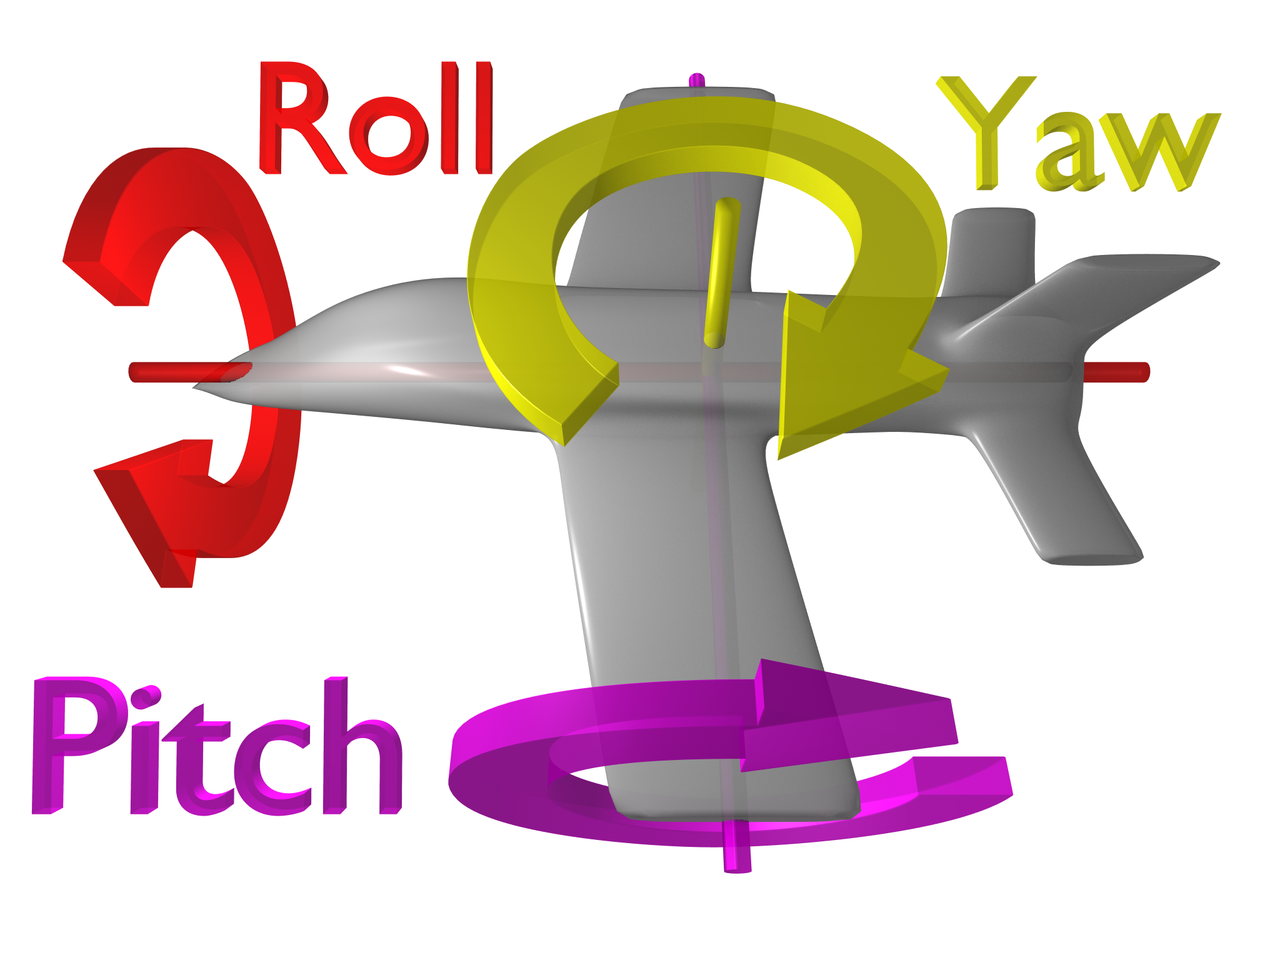
\includegraphics[width=0.5\textwidth]{airplane-axis}
    \caption{Mená osí pre letectvo.}
    \label{pic:airplaneaxis}
\end{figure}

Tento problém je možné preniesť do klasifikácie, preto pre riešenie tohto problému budú použité konvolučné neurónové siete, ktorých všeobecná architektúra je popísaná v \ref{sec:architekuraCNN}.
Výsledok poslednej vrstvy softmax klasfikátora bude 72 výstupov, ktoré budú určovať o aký uhol je zbraň natočená.
Každá zo 72 kategórií bude zastupovať rozpätie 5 stupňov, čiže celkovo sa určí náklon zbrane v celom rozsahu od 0 do 360 stupňov.

Postup predspracovania obrazu bude rovnaký ako pri klasfikácií zbraní pomocou konvolučných neurónových sietí, normalizácia, úprava rozmeru vstupu na štvorec a augmentácia dát (viď. \ref{subsec:augmentacia})
Pre každú os bude natrénovaná samostatná konvolučná neurónová sieť, výsledok bude teda obsahovať 3 natrénované modely.

\subsection{Odchýlka chyby}
\label{subsec:odchylkachyby}
Knižnica Keras obsahuje funkciu \textit{categorical\_accuracy}\footnote{\url{https://keras.io/metrics/}} pre určenie presnosti siete pri klasifikovaní do viacerých kategórií.
Čo je možné použiť, avšak pre určenie náklonu by bola vhodná iná metrika určovania presnosti siete.
Preto bude implementovaná vlastná funkcia \textit{angle\_error}, ktorá bude počítať presnosť siete podľa priemerného rozdielu medzi skutočnými a predpovedanými uhlami.
